Cai et al. \cite{caiMSTMultistageSpectralwise2022a} propose the Multi-stage Spectral-wise Transformer (MST),
for the task of spectral super resolution.
The idea the authors introduce, is instead of forming tokens by partitioning the spatial domain,
entire spectral-bands are being treated as tokens.
Given a feature map $X \in \mathbb R^{C \times H \times W}$, the spatial domain is flattened,
leading to the shape $C \times HW$,
each entry in the channel dimension is then treated as a token, 
yielding $(x_k)_{k=1}^{C} \in \mathcal S( \mathbb R^{HW})$.
The model architecture is depicted in figure \ref{fig:mst}.

\begin{figure}[h!]
    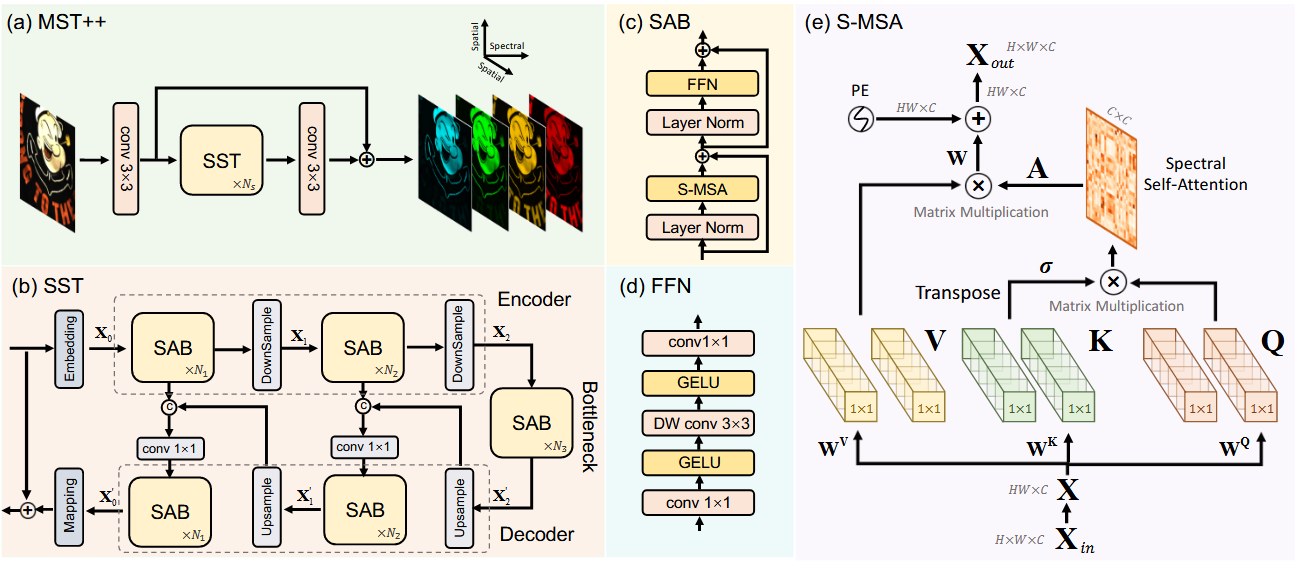
\includegraphics[width=0.9\textwidth]{models/ssr/imgs/mst.png}
    \caption{Image taken from \cite{caiMSTMultistageSpectralwise2022a}, architecture of MST model.}
    \label{fig:mst}
\end{figure}

The basic building block of the MST forms the Spectral Attention Block (SAB).
A SAB is a variation of a Transformer Block as described in definition \ref{def:transformer_block}.
Instead of standard multi-headed self-attention, spectral-wise self-attention is used.
Given an input $X \in \mathbb R^{C \times H \times W}$ tokens $(x_k)_{k = 1}^C \in \mathcal S (\mathbb R^{HW})$ are formed,
as described in the introduction.
The tokens are embedded using matrices $Q_h, K_h, V_h \in \mathbb R^{d_h \times C}$,
for $h = 1, ..., H$, as in standard multi-headed self-attention, 
to obtain provisional queries and keys $(\hat{q}_k^{(h)})_{k=1}^{HW}, (\hat{k}_k^{(h)})_{k=1}^{HW}$ 
as well as values $(\hat{v}_k^{(h)})_{k=1}^{HW} \in \mathcal{S}(\mathbb R^{C})$, that is

    \begin{equation} \label{eq:smsa1}
        \hat{q}_k^{(h)} = Q_h x_k, \hat{k}_k^{(h)} = K_h x_k \text{ and } \hat{v}_k^{(h)} = V_h x_k ~.
    \end{equation}

In contrary to standard self-attention the tokens are then transposed in some sense
\footnote{If one represents queries, keys and values as matrices, i.e. $X_Q^{(h)} = Q_hX, X_K^{(h)} = K_hX$ and $X_V^{(h)} = V_hX$ for $h = 1, ..., H$,
where $X \in \mathbb R^{C \times HW}$,
the attention scores are computed by $A_h = \text{softmax}( \sigma_h {X_K^{(h)}}^\top X_Q^{(h)}) \in \mathbb R^{C \times C}$.
Note, for standard self-attention they are computed by $A_h = \text{softmax}( \frac{1}{\sqrt{d_h}} X_Q^{(h)} {X_K^{(h)}}^\top) \in \mathbb R^{HW \times HW}$.}, 
to obtain the final queries, keys $(q_k^{(h)})_{k=1}^{C}, (k_k^{(h)})_{k=1}^{C}$ and values $(v_k^{(h)})_{k=1}^{C} \in \mathcal{S} (\mathbb R^{HW})$
given by

    \begin{equation} \label{eq:smsa2}
        q_k^{(h)}(i) = \hat{q}_i^{(h)}(k) ~, ~~ k_k^{(h)}(i) = \hat{k}_i^{(h)}(k) \text{ and } v_k^{(h)}(i) = \hat{v}_i^{(h)}(k) ~,
    \end{equation}

for $i = 1, ..., HW$ and $k = 1, ..., C$.
To the computation of attention scores an optimizable scalar $\sigma_j \in \mathbb R$ is introduced,
replacing by the factor $\frac{1}{\sqrt{d}}$ commonly used. 
The authors report that spectral density varies strongly with respect to the wavelength,
which is thereby accounted for

    \begin{equation} \label{eq:smsa3}
        A_{ij}^{(h)} = \frac{\text{exp} \left( \sigma_j {k_{i}^{(h)}}^\top q_{j}^{(h)} \right)}{\sum_{k = 1}^n \text{exp} \left( \sigma_j {k_{k}^{(h)}}^\top q_{j}^{(h)} \right)}
    \end{equation}

for $i, j = 1, ..., d_h$.
Finally the values are weighted by the attention scores

    \begin{equation} \label{eq:smsa4}
        \hat{y}_j^{(h)} = \sum_{i=1}^{C} A_{ij}^{(h)} v_j^{(h)} ~,
    \end{equation}

Using an optimizable matrix $W \in \mathbb R^{C \times C}$, 
the heads are merged back together 

    \begin{equation} \label{eq:smsa5}
        \hat{y}_k = W [\hat{y}_k^{(1)}, ..., \hat{y}_k^{(H)}] ~,
    \end{equation}

for $k = 1, ..., HW$. 
One more peculiar design choice the authors made,
positional encodings are added as a last step and computed using a shallow network $\phi$ from the value embeddings $\hat{v}_k$,
that is 

    \begin{equation} \label{eq:smsa6}
        y_k = \hat{y}_k + \phi \left( \big[\hat{v}_k^{(1)}, ..., \hat{v}_k^{(H)}] \right) ~,
    \end{equation}

where $\phi$ is defined by

    \begin{equation*}
        \phi = F(H \cdot W, H \cdot W) \circ \text{GELU} \circ F(H \cdot W, H \cdot W) ~.
    \end{equation*}

The difference between spectral and standard self-attention is visualized once more in figure \ref{fig:smsa}.

\begin{figure}[h!]
    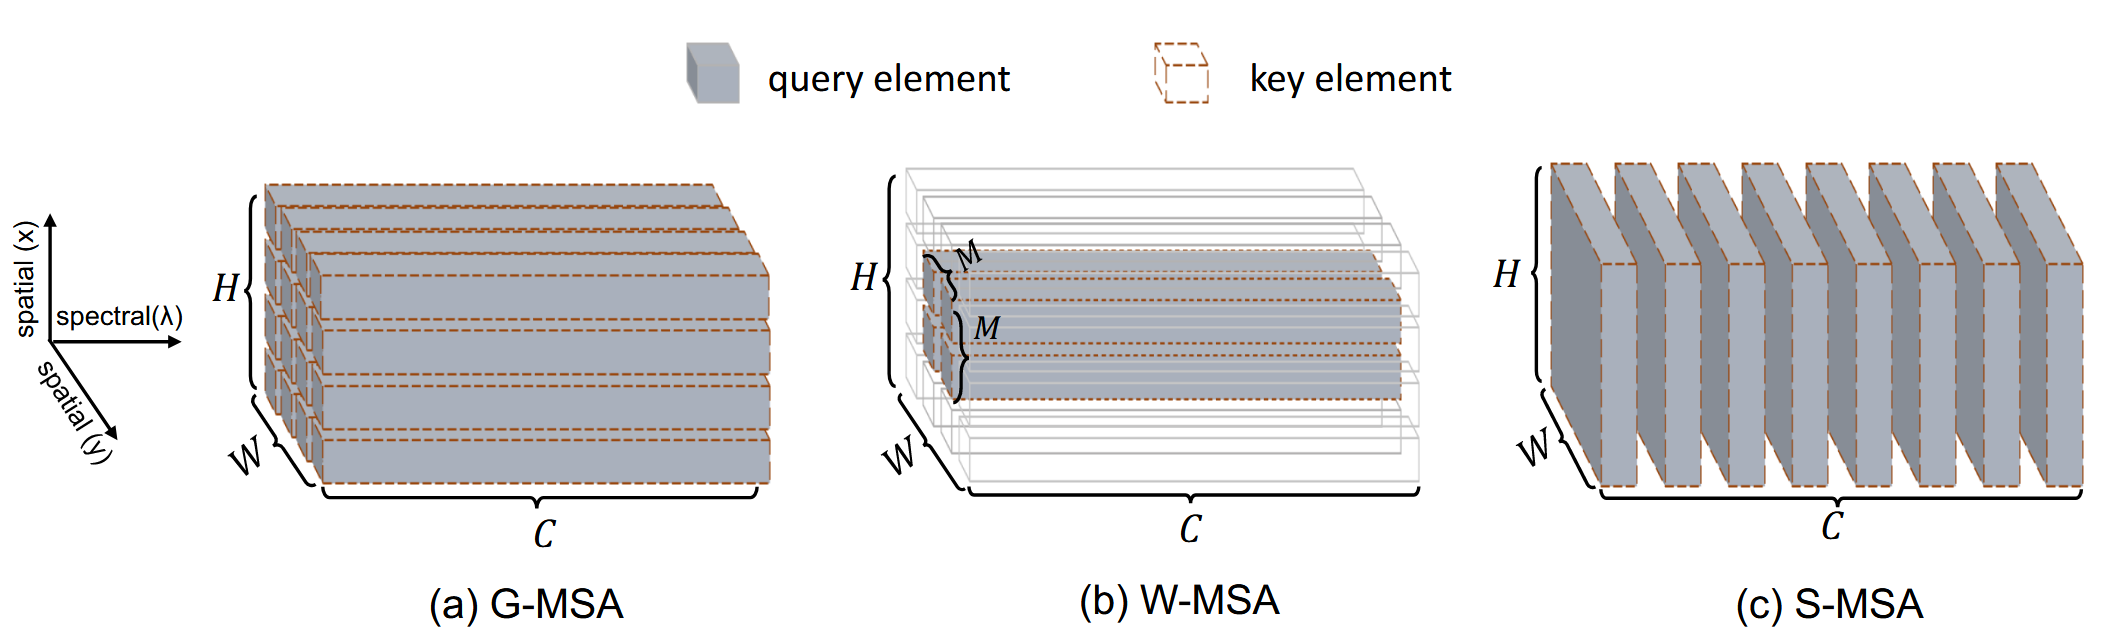
\includegraphics[width=0.9\textwidth]{models/ssr/imgs/smsa.png}
    \caption{Image taken from \cite{caiMSTMultistageSpectralwise2022a}, Spectral Multi-headed Self-Attention.}
    \label{fig:smsa}
\end{figure}

We capture the operation in the following definition.

\begin{definition}[Spectral Multi-headed Self-Attention]
    The operation defined through equations (\ref{eq:smsa1}), (\ref{eq:smsa2}), (\ref{eq:smsa3}), (\ref{eq:smsa4}), (\ref{eq:smsa5}) and (\ref{eq:smsa6})

        \begin{equation*}
            \text{S-MSA} : \mathcal{S}( \mathbb{R}^d) \to \mathcal{S}( \mathbb{R}^d) ~, ~~ \text{S-MSA} \left( (x_k)_{k = 1}^N \right) = (y_k)_{k = 1}^N ~,
        \end{equation*}

    is called Spectral Multi-Headed Self-Attention.
\end{definition}

As already mentioned in the beginning, the Spectral Multi-Headed Self-Attention Block $H_{SAB}$ is a variation of the transformer block

\begin{equation*}
    H_{SAB} = R( \phi \circ \text{LN} ) \circ R( \text{S-MSA} \circ \text{LN} ) ~,
\end{equation*}

here $\phi : \mathbb R^{C \times H \times W} \to \mathbb R^{C \times H \times W}$ is defined as a three layer CNN

\begin{equation*}
    \phi = C(4d, d, \text{kernel-size}=1) \circ \text{GELU} \circ C(4d, 4d, \text{kernel-size}=3, \text{padding}=1) \circ \text{GELU} \circ C(d, 4d, \text{kernel-size}=1) ~.
\end{equation*}

We have introduced the SAB, we can now move on to describe how the architecture builds upon this module.
The deep feature extraction module $H_d$ consists of $3$ cascaded Single-stage Spectral-wise Transformers (SSTs),
followed by a final convolutional layer

    $$ H_d = C \circ H_{SST} \circ ... \circ H_{SST} ~. $$

An SST admits a U-Net like architecture, displayed in part (b) of figure \ref{fig:mst}.
In order to describe an SST we are missing the downsampling and upsampling modules.
The downsampling module is given by a strided convolution

    \begin{equation*}
        H_{down}(d_{in}, d_{out}) = C(d_{in}, d_{out}, \text{kernel-size}=4, \text{stride}=2, \text{padding}=1) ~,
    \end{equation*}

whereas upsampling is achieved using a transposed convolution

    \begin{equation*}
        H_{up}(d_{in}, d_{out}) = C^\top(d_{in}, d_{out}, \text{kernel-size}=2, \text{stride}=2, \text{padding}=0) ~.
    \end{equation*}

Given initial features $F_0 \in \mathbb R^{31 \times H \times W}$, 
these are first processed using a convolutional layer

    \begin{equation*}
        F_1 = C(31, 31, \text{kernel-size}=3, \text{padding}=1)(F_0) ~.
    \end{equation*}

The features are then passed through the contracting path,
were they are processed using a SAB followed by downsampling

    \begin{equation*}
        F_i = H_{down}(2^{i-1} \cdot 31, 2^i \cdot 31) \circ H_{SAB}(2^{i-1} \cdot 31, H)(F_{i-1}) ~,
    \end{equation*}

for $i=2, 3$. Next, the features undergo the bottleneck, which consists of a single SAB

    \begin{equation*}
        F_4 = H_{SAB}(122, H)(F_{3}) ~.
    \end{equation*}

Afterwards the features are passed through the expanding path, 
as it is common practice in U-Net architectures,
features from the same levels are concatenated

    \begin{equation*}
        F_i =  H_{up}(2^{7 - i} \cdot 31, 2^{6 - i} \cdot 31) \circ H_{SAB}(2^{7-1} \cdot 31, H) \left( \big[F_{i-1}, (F_{8 - i}) \big] \right) ~,
    \end{equation*}

for $i = 5, 6$.
The features are then passed through a final convolutional layer

    \begin{equation*}
       F_1 = C(31, 31, \text{kernel-size}=3, \text{padding}=1)(F_0) ~.
    \end{equation*}

This is the final output of the SST module.